\documentclass[conference, a4paper]{IEEEtran}

% Υποστήριξη Ελληνικών για pdflatex
\usepackage[utf8]{inputenc}
\usepackage[english,greek]{babel}
\usepackage[LGR,T1]{fontenc}
\usepackage{alphabeta}

% Χρήση της προεπιλεγμένης γραμματοσειράς του LaTeX (Latin Modern / Computer Modern)
\usepackage{lmodern}
\usepackage{amsmath}

% Redefine IEEEtran keywords name to Greek
\renewcommand{\IEEEkeywordsname}{Λέξεις Κλειδιά}

\makeatletter
\def\abstract{
    \if@twocolumn
      \@IEEEabskeysecsize\textit{\abstractname}\ \relax
    \else
      \bgroup\par\addvspace{0.5\baselineskip}\centering\vspace{-1.78ex}\@IEEEabskeysecsize\textbf{\abstractname}\par\addvspace{0.5\baselineskip}\egroup\quotation\@IEEEabskeysecsize\normalfont
    \fi\@IEEEgobbleleadPARNLSP}
\def\IEEEkeywords{
    \if@twocolumn
      \@IEEEabskeysecsize\textit{\IEEEkeywordsname}\ \relax
    \else
      \bgroup\par\addvspace{0.5\baselineskip}\centering\@IEEEabskeysecsize\textbf{\IEEEkeywordsname}\par\addvspace{0.5\baselineskip}\egroup\quotation\@IEEEabskeysecsize\normalfont
    \fi\@IEEEgobbleleadPARNLSP}
\makeatother

% Μαθηματικά πακέτα
\usepackage{amsmath, amssymb, amsfonts}
\usepackage{graphicx}
\usepackage{booktabs}
\usepackage{hyperref}

\begin{document}

\title{\textlatin{Interpretable World Models Principles}}

\author{\IEEEauthorblockN{Φ. Πλουμής \quad Α. Ρήγας \quad Η. Μπακογιώργος \quad Α. Φειδάκης}
\IEEEauthorblockA{\textit{Σχολή Ηλεκτρολόγων Μηχανικών \& Μηχανικών Υπολογιστών} \\
\textit{Εθνικό Μετσόβιο Πολυτεχνείο}, Αθήνα}
}

\maketitle

\begin{abstract}
Η παρούσα εργασία παρουσιάζει την αναπαραγωγή και εκτεταμένη αξιολόγηση των αρχών σχεδιασμού για \textlatin{World Models} (\textlatin{PIWM}). Ενώ η αρχική μελέτη περιορίστηκε σε καθαρά περιβάλλοντα, η υλοποίησή μας αναβαθμίζει την αρχιτεκτονική (χρήση \textlatin{residual LSTMs}, \textlatin{curriculum learning}, \textlatin{scheduled sampling}) και εξετάζει την ευρωστία των μοντέλων σε συνθήκες εκτός κατανομής (\textlatin{Out-of-Distribution}, \textlatin{OOD}), όπως χωρικός θόρυβος και μεταβολές φωτεινότητας. Τα πειράματα στα περιβάλλοντα \textlatin{CartPole} και \textlatin{LunarLander} αναδεικνύουν άγνωστους περιορισμούς: η Αρχή 1 (αποσύνδεση αναπαραστάσεων) λειτουργεί ως ισχυρό φίλτρο χωρικού θορύβου, η Αρχή 2 (\textlatin{equivariance}) καταρρέει υπό τυχαίο θόρυβο αλλά διαπρέπει σε μεταβολές φωτεινότητας, ενώ η Αρχή 3 (ασθενής επίβλεψη) λειτουργεί ως έμμεση κανονικοποίηση, καθιστώντας το μοντέλο πιο ανθεκτικό από τα πλήρως επιβλεπόμενα \textlatin{baselines}. Υλοποιούμε επίσης την Αρχή 4 (διαμέριση εξόδου), επιτυγχάνοντας μείωση των παραμέτρων του \textlatin{decoder} κατά $75\%$ χωρίς απώλεια ποιότητας. Τέλος, ως επέκταση πέρα από το αρχικό άρθρο, αντικαθιστούμε το «μαύρο κουτί» \textlatin{LSTM} με αραιή ταυτοποίηση δυναμικής (\textlatin{SINDy}), η οποία ανακτά ρητές, ερμηνεύσιμες εξισώσεις κίνησης και επιδεικνύει σημαντικά μεγαλύτερη ευρωστία στον θόρυβο.
\end{abstract}

\begin{IEEEkeywords}
\textlatin{World Models, Variational Autoencoders, LSTMs, Representation Learning, Out-of-Distribution Robustness}
\end{IEEEkeywords}

\section{\textbf{Εισαγωγή}}
\label{sec:intro}

Τα \textlatin{World Models} επιτρέπουν σε πράκτορες να μαθαίνουν ένα λανθάνον (\textlatin{latent}) μοντέλο δυναμικής του περιβάλλοντός τους. Η πρόσφατη βιβλιογραφία (\textlatin{PIWM}) προτείνει τέσσερις αρχές σχεδιασμού για την ενσωμάτωση φυσικής γνώσης: (1) αποσύνδεση φυσικής και οπτικής κατάστασης, (2) επιβολή ισοδυναμίας (\textlatin{equivariance}) σε μετασχηματισμούς, (3) ασθενή επίβλεψη ταχύτητας, και (4) διαμέριση του \textlatin{decoder} ανά αντικείμενο της σκηνής.

Στην παρούσα εργασία, δεν αναπαράγουμε απλώς τα αποτελέσματα, αλλά επεκτείνουμε τη μεθοδολογία. Εντοπίσαμε ότι ο κώδικας της αρχικής δημοσίευσης υστερούσε σε σταθερότητα κατά το \textlatin{rollout}. Εισάγουμε μια αναβαθμισμένη αρχιτεκτονική και, το σημαντικότερο, εισάγουμε \textlatin{OOD} παρεμβολές (\textlatin{Gaussian/Salt \& Pepper noise}, \textlatin{brightness jitter}). Αποδεικνύουμε ότι οι αρχές αυτές δεν προσφέρουν πλεονέκτημα σε καθαρά περιβάλλοντα (όπου το \textlatin{Baseline} υπερτερεί λόγω μεγαλύτερης χωρητικότητας), αλλά αποτελούν στοχευμένους μηχανισμούς άμυνας ενάντια σε συγκεκριμένες οπτικές αλλοιώσεις. Ως επέκταση πέρα από το άρθρο, αντικαθιστούμε το \textlatin{LSTM} με αραιή ταυτοποίηση δυναμικής (\textlatin{SINDy}), δείχνοντας ότι ο φυσικά ερμηνεύσιμος λανθάνων χώρος επιτρέπει την εξαγωγή ρητών εξισώσεων κίνησης με αυξημένη ευρωστία.

\section{\textbf{Μεθοδολογία και Υλοποίηση}}
\label{sec:method}

Η προτεινόμενη αρχιτεκτονική υλοποιεί ένα μοντέλο \textlatin{two-stage}. Αρχικά, ένας \textlatin{Variational Autoencoder} (\textlatin{VAE}) χρησιμοποιείται για την εξαγωγή συμπαγών λανθανόντων χαρακτηριστικών $z_t$ από υψηλής διάστασης οπτικές παρατηρήσεις $o_t$. Στη συνέχεια, ένα αναδρομικό νευρωνικό δίκτυο (\textlatin{LSTM}) αναλαμβάνει την πρόβλεψη της μελλοντικής δυναμικής $\hat{z}_{t+1} = f(z_t, a_t)$, δεδομένης της τρέχουσας κατάστασης και της δράσης $a_t$ του πράκτορα.

\subsection{\textbf{Αναβαθμίσεις Αρχιτεκτονικής Δυναμικής (\textlatin{LSTM})}}
Για να αποτρέψουμε την κατάρρευση των προβλέψεων σε μεγάλους ορίζοντες (π.χ. $h=30$), υλοποιήσαμε \textlatin{Residual LSTMs}, όπου το δίκτυο μαθαίνει τη μεταβολή της κατάστασης:
\begin{equation}
    \hat{z}_{t+1} = z_t + \text{\textlatin{LSTM}}(z_t, a_t; \theta)
\end{equation}
Επιπλέον, ενσωματώσαμε \textlatin{Curriculum Learning} (σταδιακή αύξηση του ορίζοντα εκπαίδευσης) και \textlatin{Scheduled Sampling} (εκθετική μείωση του \textlatin{teacher forcing}), στοιχεία που απουσίαζαν από την αρχική υλοποίηση.

\subsection{\textbf{Αρχή 1: Αποσύνδεση (\textlatin{Disentanglement})}}
Η Αρχή 1 επιβάλλει τη δομική αποσύνδεση του \textlatin{VAE} σε έναν \textlatin{encoder} για τη φυσική κατάσταση $z_{\text{\textlatin{phys}}} \in \mathbb{R}^k$ (π.χ. $k=4$ για το \textlatin{CartPole}) και έναν για το οπτικό στυλ $z_{\text{\textlatin{img}}}$. Η συνάρτηση απώλειας περιλαμβάνει την τυπική \textlatin{ELBO}, με την επιπλέον συνθήκη ότι η ανακατασκευή χρησιμοποιεί τον διαχωρισμένο χώρο.

\subsection{\textbf{Αρχή 2: Ισοδυναμία (\textlatin{Equivariance})}}
Η Αρχή 2 χρησιμοποιεί έναν ενιαίο/μονολιθικό \textlatin{encoder} (όπως το \textlatin{Baseline}) αλλά επιβάλλει κανονικοποίηση ισοδυναμίας. Αν $g$ είναι ένας μετασχηματισμός στην εικόνα (π.χ. αλλαγή φωτεινότητας) και $h$ ο αντίστοιχος μετασχηματισμός στον λανθάνοντα χώρο, ελαχιστοποιείται η απόσταση:
\begin{equation}
    \textlatin{\ensuremath{\mathcal{L}}}_{\text{\textlatin{eq}}} = \mathbb{E}_{o \sim D} \left[ || E(g \cdot o) - h \cdot E(o) ||_2^2 \right]
\end{equation}
Στην περίπτωση της φωτεινότητας, το $h$ είναι ο ταυτοτικός μετασχηματισμός (\textlatin{invariance}).

\subsection{\textbf{Αρχή 3: Ασθενής Επίβλεψη (\textlatin{Weak Supervision})}}
Συχνά η πραγματική ταχύτητα (\textlatin{velocity}) δεν είναι διαθέσιμη. Υλοποιήσαμε την Αρχή 3 υπολογίζοντας προσεγγιστικές ταχύτητες μέσω πεπερασμένων διαφορών:
\begin{equation}
    v_t \approx \frac{x_{t+1} - x_t}{\Delta t}
\end{equation}
Αυτές οι «θορυβώδεις» εκτιμήσεις χρησιμοποιούνται για την επίβλεψη των διαστάσεων ταχύτητας στον λανθάνοντα χώρο.

\subsection{\textbf{Αρχή 4: Διαμέριση Εξόδου (\textlatin{Compositional Decoding})}}
Αντί ενός μονολιθικού \textlatin{decoder}, η Αρχή 4 χρησιμοποιεί ανεξάρτητους αποκωδικοποιητές ανά αντικείμενο της σκηνής (π.χ. \textlatin{cart}, \textlatin{pole}, \textlatin{background}), των οποίων οι έξοδοι συντίθενται στην τελική εικόνα. Η διάσπαση αυτή μειώνει δραστικά τις παραμέτρους του \textlatin{decoder} και επιτρέπει την επαλήθευση ανά συνιστώσα.

\subsection{\textbf{Επέκταση: Ερμηνεύσιμη Δυναμική με \textlatin{SINDy}}}
Πέρα από το αρχικό άρθρο, εξετάζουμε αν η δυναμική του (φυσικά εποπτευόμενου) λανθάνοντος χώρου μπορεί να ταυτοποιηθεί \emph{ρητά}. Εφαρμόζουμε \textlatin{SINDYc} (\textlatin{Sparse Identification of Nonlinear Dynamics with control})~\cite{sindy} στις φυσικές διαστάσεις, μαθαίνοντας έναν αραιό πίνακα συντελεστών $\Xi$ πάνω σε μια βιβλιοθήκη υποψήφιων συναρτήσεων $\Theta(z,u)$ (πολυώνυμα, τριγωνομετρικοί όροι, συζεύξεις ελέγχου):
\begin{equation}
    \hat{z}_{t+1} = z_t + \Theta(z_t, u_t)\,\Xi ,
\end{equation}
όπου το $\Xi$ προκύπτει μέσω \textlatin{Sequentially Thresholded Least Squares} (\textlatin{STLSQ}). Δοκιμάζουμε επίσης ένα \textlatin{gray-box hybrid}, όπου ένα υπολειμματικό \textlatin{LSTM} διορθώνει το (παγωμένο) \textlatin{SINDy}: $\hat{z}_{t+1} = z_t + \Theta(z_t,u_t)\Xi + \text{\textlatin{LSTM}}(z_t,a_t)$.

\section{\textbf{Πειραματική Διάταξη}}
\label{sec:setup}

Τα πειράματα διεξήχθησαν σε δύο περιβάλλοντα: το κλασικό \textlatin{CartPole} και το πιο πολύπλοκο \textlatin{LunarLander}.
Λόγω της \textlatin{heavy-tail} κατανομής των σφαλμάτων πρόβλεψης σε μεγάλους ορίζοντες, η αξιολόγηση έγινε χρησιμοποιώντας δείκτες ευρωστίας: διάμεσο (\textlatin{Median}) και ενδοτεταρτημοριακό εύρος (\textlatin{IQR}). Για τη σύγκριση μοντέλων ($A$ vs $B$), υπολογίσαμε την κατά ζεύγη διαφορά (\textlatin{Paired Difference}) $\Delta = \text{\textlatin{MSE}}_{\textlatin{A}} - \text{\textlatin{MSE}}_{\textlatin{B}}$ με 95\% \textlatin{Bootstrap Confidence Intervals} ($N=1000$ \textlatin{resamples}).

\section{\textbf{Αποτελέσματα}}
\label{sec:results}

\subsection{\textbf{Αξιολόγηση σε Καθαρά Περιβάλλοντα}}
Σε περιβάλλοντα χωρίς οπτικό θόρυβο ($\sigma=0$), το απλό \textlatin{Baseline} μοντέλο τείνει να υπερτερεί ή να ισοβαθμεί με τις Αρχές 1 και 2. Όπως φαίνεται στο Σχήμα \ref{fig:clean_env}, η μέση τετραγωνική απόσταση (\textlatin{State MSE}) για το \textlatin{Baseline} και την Αρχή 2 είναι εξαιρετικά χαμηλή και σχεδόν ταυτόσημη. Αντίθετα, η Αρχή 1 παρουσιάζει ελαφρώς μεγαλύτερο σφάλμα. Αυτό εξηγείται διότι, χωρίς \textlatin{distractors}, οι αρχιτεκτονικοί περιορισμοί (όπως το στενό \textlatin{bottleneck} των 4 διαστάσεων της Αρχής 1) απλώς περιορίζουν τη χωρητικότητα του δικτύου. Αυτό επιβεβαιώνει ότι οι αρχές του \textlatin{PIWM} δεν προσφέρουν απαραίτητα βελτίωση της ακρίβειας σε ιδανικές συνθήκες, αλλά αποσκοπούν στην ευρωστία.

\begin{figure}[h]
    \centering
    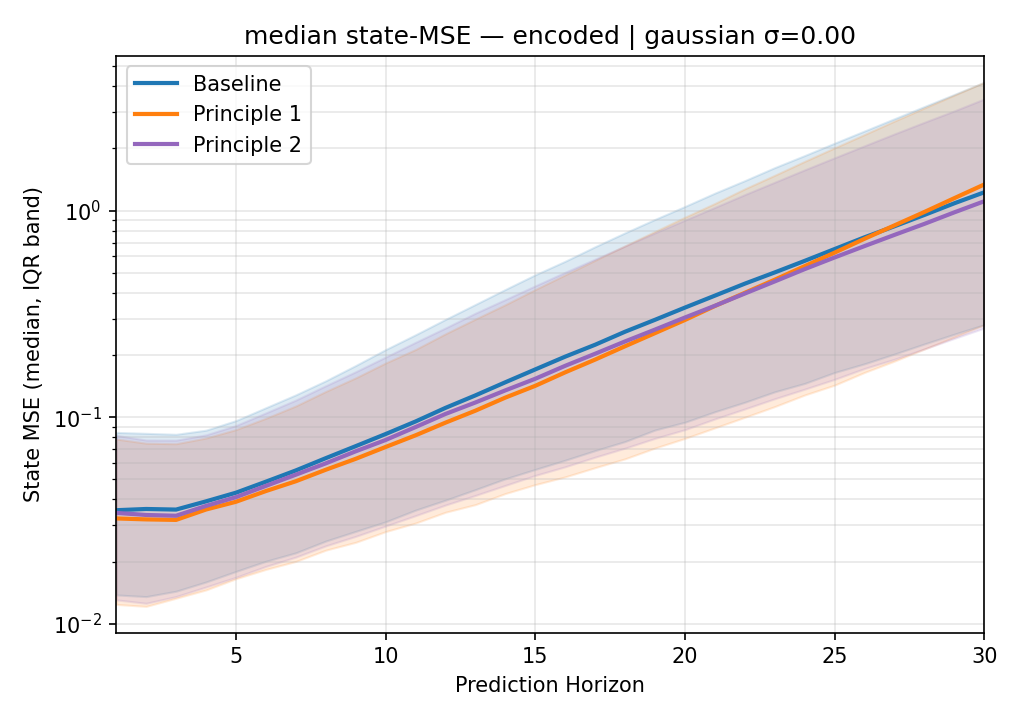
\includegraphics[width=\linewidth]{pics/noise_median_iqr_encoded_gaussian_0p00_p1_p2.png}
    \caption{Αναπαραγωγή των αποτελεσμάτων του \textlatin{PIWM} σε απόλυτα καθαρό περιβάλλον (\textlatin{encoded state, $\sigma=0.00$}). Τα μοντέλα \textlatin{Baseline} και Αρχή 2 ταυτίζονται σχεδόν απόλυτα, ενώ η Αρχή 1 εμφανίζει ελαφρώς χειρότερη απόδοση λόγω δομικών περιορισμών.}
    \label{fig:clean_env}
\end{figure}

\subsection{\textbf{Αρχή 1: Δομικό Φίλτρο Χωρικού Θορύβου}}
Κατά την εισαγωγή \textlatin{Gaussian noise}, η Αρχή 1 επέδειξε εντυπωσιακή ευρωστία. Σε ορίζοντα προβλέψεων $h=30$ και έντονο θόρυβο $\sigma=0.30$, το \textlatin{MSE} της Αρχής 1 διατηρήθηκε σε χαμηλά επίπεδα, εν αντιθέσει με το \textlatin{Baseline} και την Αρχή 2 που παρουσίασαν πλήρη κατάρρευση (βλ. Σχήμα \ref{fig:p1_noise}).

\begin{figure}[h]
    \centering
    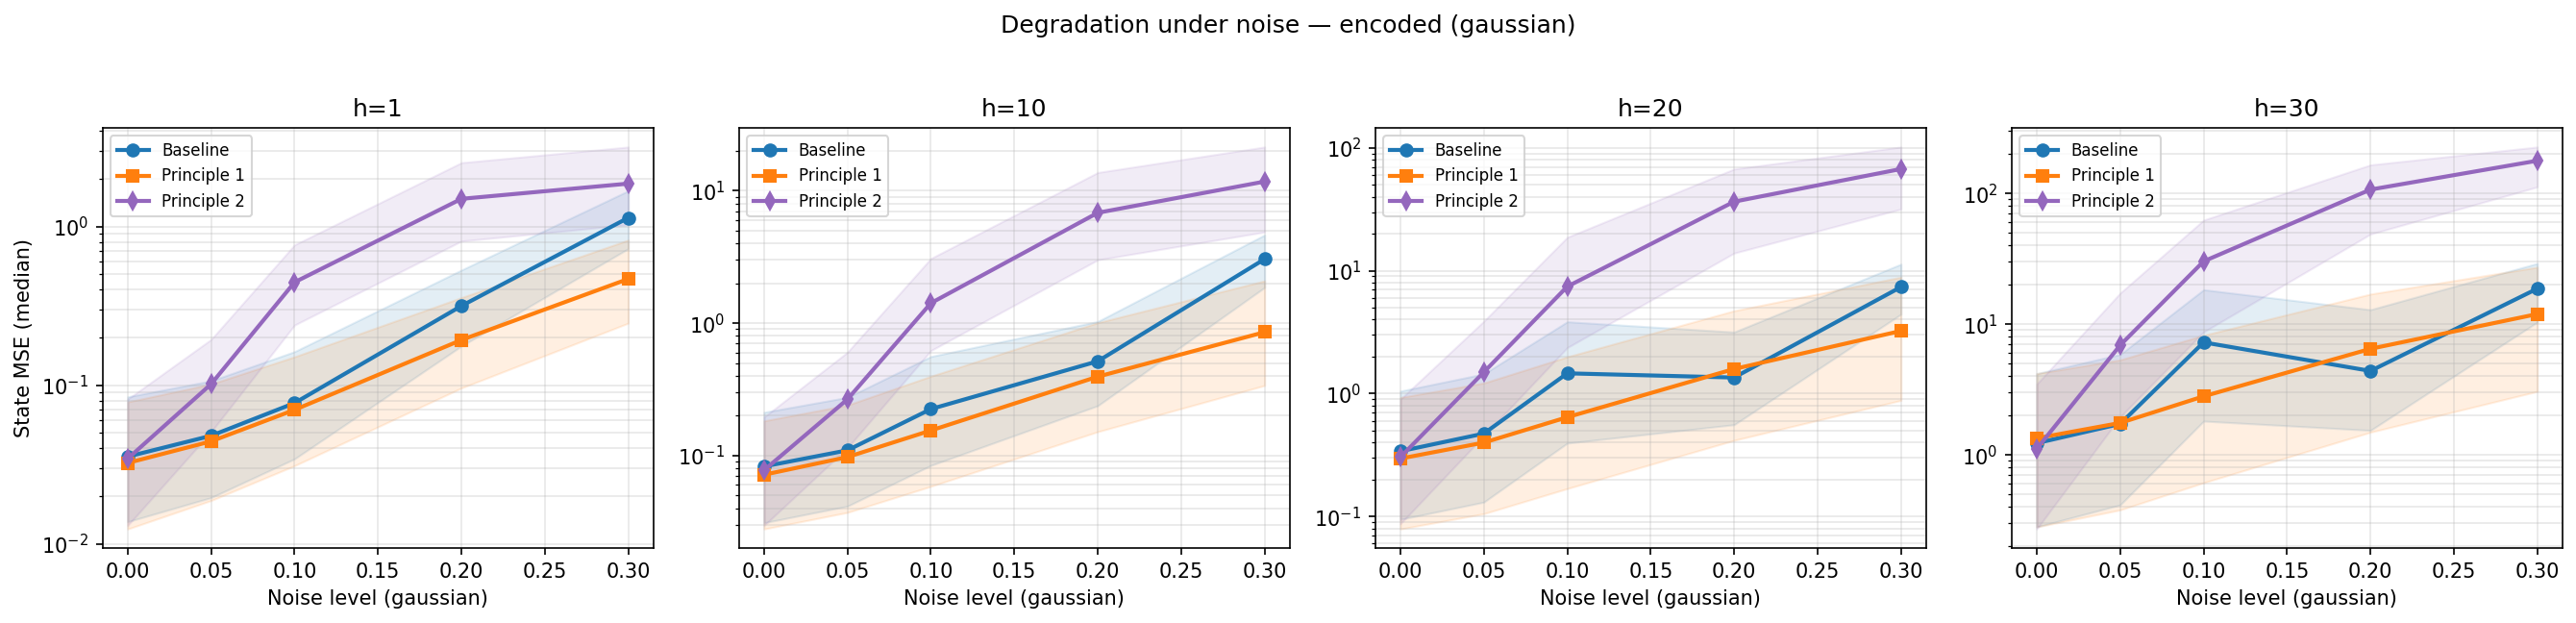
\includegraphics[width=\linewidth]{pics/noise_degradation_encoded_gaussian.png}
    \caption{Αξιολόγηση ευρωστίας (\textlatin{State MSE}) σε διαφορετικά επίπεδα \textlatin{Gaussian Noise} για το περιβάλλον \textlatin{CartPole}. Διακρίνεται η υπεροχή της Αρχής 1 (πορτοκαλί καμπύλη) σε υψηλά επίπεδα θορύβου.}
    \label{fig:p1_noise}
\end{figure}

Η συμπεριφορά αυτή εξηγείται θεωρητικά από τη δομή του \textlatin{VAE}. Ο διαχωρισμός του \textlatin{encoder} δρα ως φυσικό φίλτρο: ο μη-δομημένος θόρυβος των \textlatin{pixels} αδυνατεί να βρει συσχέτιση με τις παραμέτρους της δυναμικής του συστήματος και εγκλωβίζεται σχεδόν εξ ολοκλήρου στον \textlatin{encoder} του στυλ ($z_{\text{\textlatin{img}}}$). Ως αποτέλεσμα, δεν «μολύνει» τις φυσικές διαστάσεις ($z_{\text{\textlatin{phys}}}$), προστατεύοντας τις προβλέψεις του \textlatin{LSTM}.

\subsection{\textbf{Αρχή 2: Το Κόστος της Κανονικοποίησης}}
Τα πειράματά μας αποκάλυψαν τον διττό χαρακτήρα της Αρχής 2. Από τη μία πλευρά, διαπρέπει απέναντι σε συστηματικές αλλαγές φωτεινότητας (\textlatin{brightness jitter}). Όπως φαίνεται στο Σχήμα \ref{fig:p2_brightness}, η στατιστική ανάλυση \textlatin{bootstrap} της κατά ζεύγη διαφοράς (\textlatin{Paired Difference}) επιβεβαιώνει με 95\% διάστημα εμπιστοσύνης ότι η Αρχή 2 υπερτερεί σταθερά του \textlatin{Baseline} σε αυτά τα πειράματα.

\begin{figure}[h]
    \centering
    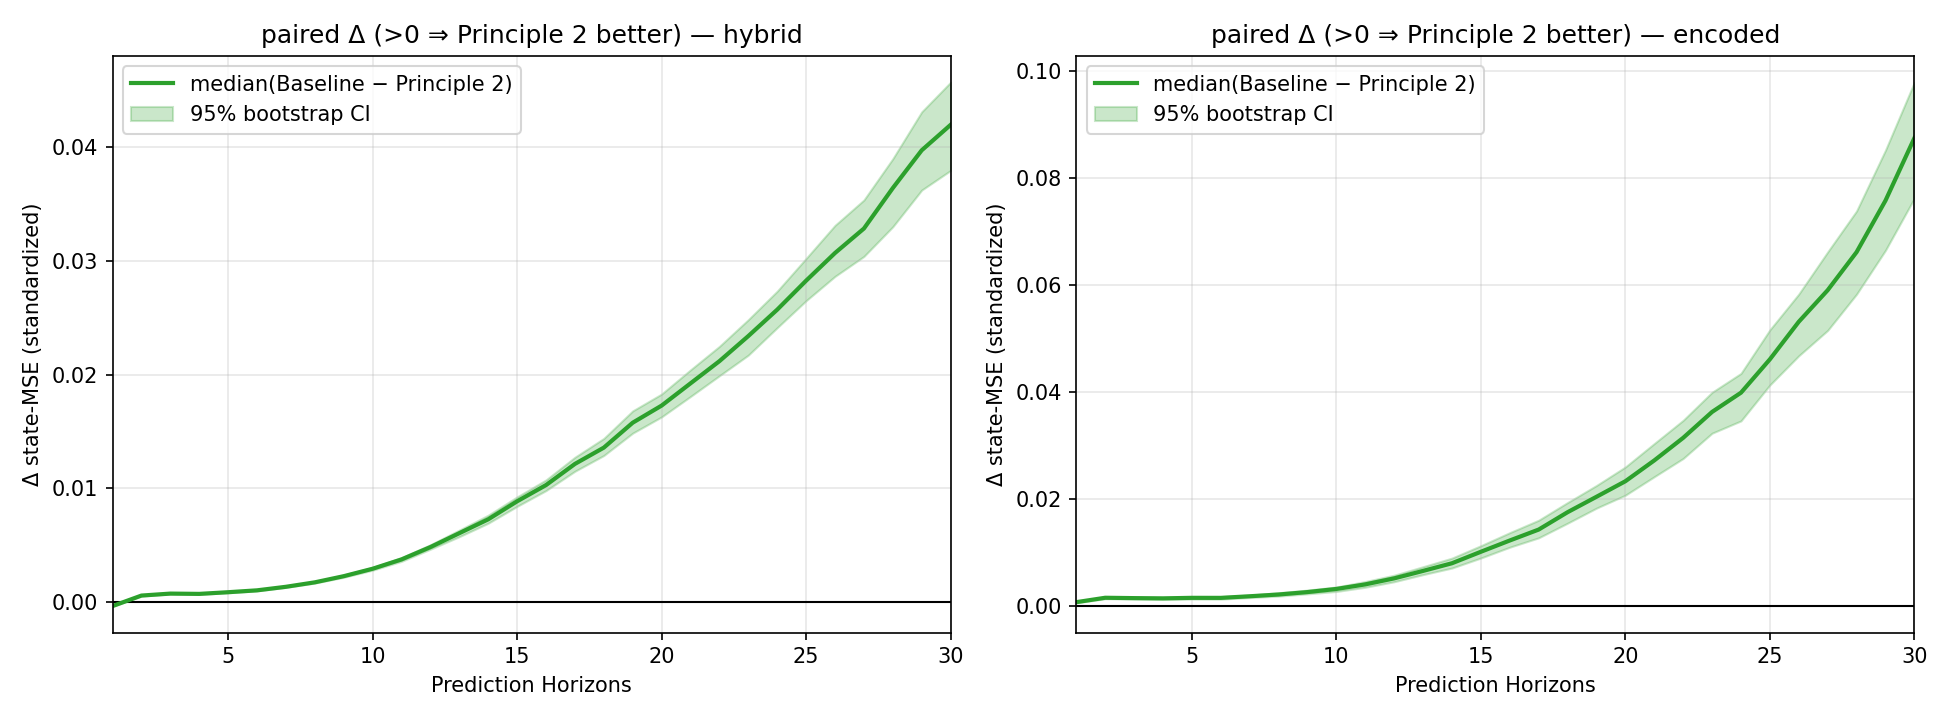
\includegraphics[width=\linewidth]{pics/cmp_paired_diff.png}
    \caption{Ανάλυση \textlatin{Paired Difference} ($\Delta = \text{\textlatin{Baseline}} - \text{\textlatin{Principle 2}}$) υπό συνθήκες \textlatin{Brightness Jitter}. Η θετική διαφορά επιβεβαιώνει την ανωτερότητα της Αρχής 2.}
    \label{fig:p2_brightness}
\end{figure}

Από την άλλη πλευρά, ωστόσο, η Αρχή 2 αποτυγχάνει παταγωδώς υπό χωρικό θόρυβο. Εικάζουμε ότι η ισχυρή κανονικοποίηση \textlatin{equivariance} αναγκάζει το μοντέλο να εστιάσει υπερβολικά στις ακριβείς ακμές και στις χωρικές οπτικές δομές της εικόνας για να ικανοποιήσει την εξίσωση (2). Όταν αυτές οι δομές καταστρέφονται από τυχαίο θόρυβο επιπέδου \textlatin{pixel}, ο μονολιθικός \textlatin{encoder} αδυνατεί να γενικεύσει και παράγει ακραίες \textlatin{OOD} αναπαραστάσεις, αποσταθεροποιώντας πλήρως το \textlatin{LSTM}.

\subsection{\textbf{Αρχή 3: Η Ατέλεια ως Κανονικοποίηση (\textlatin{Implicit Regularization})}}
Στην περίπτωση της Αρχής 3, παρατηρήσαμε ένα παράδοξο. Σε καθαρά περιβάλλοντα (Σχήμα \ref{fig:p3_clean}), το πλήρως επιβλεπόμενο \textlatin{Baseline} τείνει να υπερτερεί έναντι των μοντέλων με ασθενή επίβλεψη (\textlatin{P3-weak}) ή μερική επίβλεψη (\textlatin{P3-semi}). 

\begin{figure}[h]
    \centering
    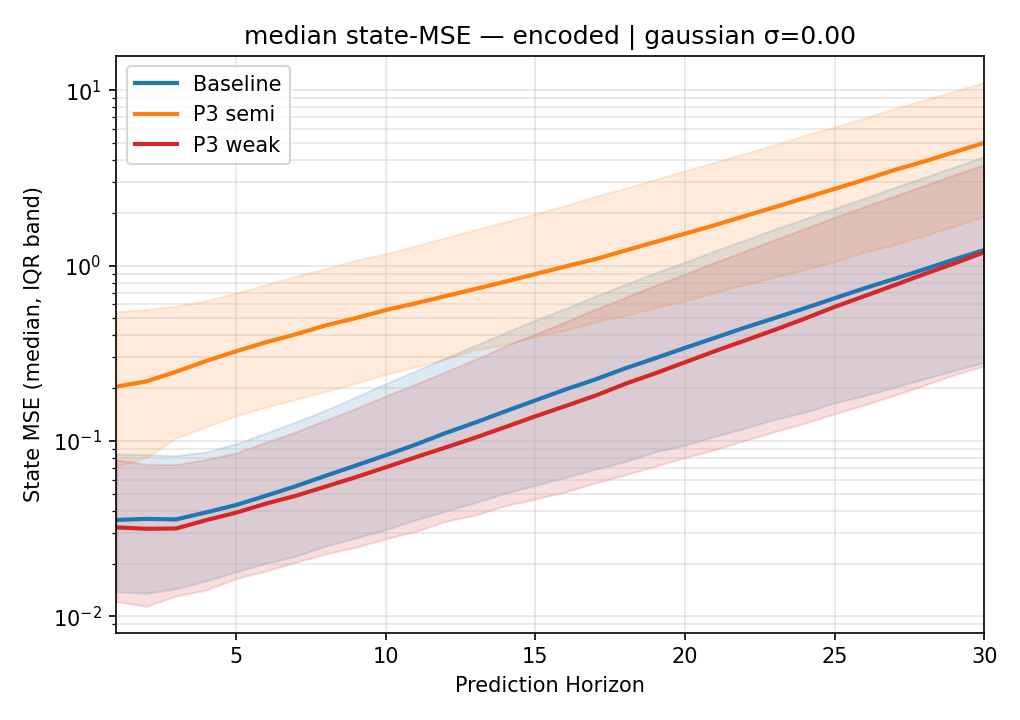
\includegraphics[width=\linewidth]{pics/noise_median_iqr_encoded_gaussian_0p00_p3.png}
    \caption{Αναπαραγωγή αποτελεσμάτων της Αρχής 3 σε καθαρό περιβάλλον ($\sigma=0.00$). Το πλήρως επιβλεπόμενο \textlatin{Baseline} είναι το πιο ακριβές, ενώ η απουσία επίβλεψης ταχύτητας (\textlatin{P3-semi}) οδηγεί σε μεγαλύτερο σφάλμα.}
    \label{fig:p3_clean}
\end{figure}

Ωστόσο, το μοντέλο \textlatin{P3-weak} (ασθενής επίβλεψη μέσω πεπερασμένων διαφορών) αποδείχθηκε πιο ανθεκτικό στον οπτικό θόρυβο από το \textlatin{Baseline} (Σχήμα~\ref{fig:p3_noise}). Καθώς εκπαιδεύτηκε με «θορυβώδεις» εκτιμήσεις ταχύτητας, ο λανθάνων χώρος του δεν έκανε \textlatin{overfit} στην ψευδαίσθηση των τέλειων δεδομένων, δρώντας ως \textlatin{implicit regularizer}. Αντίθετα, το \textlatin{P3-semi} (καμία επίβλεψη ταχύτητας) απέτυχε πλήρως υπό θόρυβο, επιβεβαιώνοντας ότι κάποια μορφή δυναμικής γνώσης είναι απαραίτητη.

\begin{figure}[h]
    \centering
    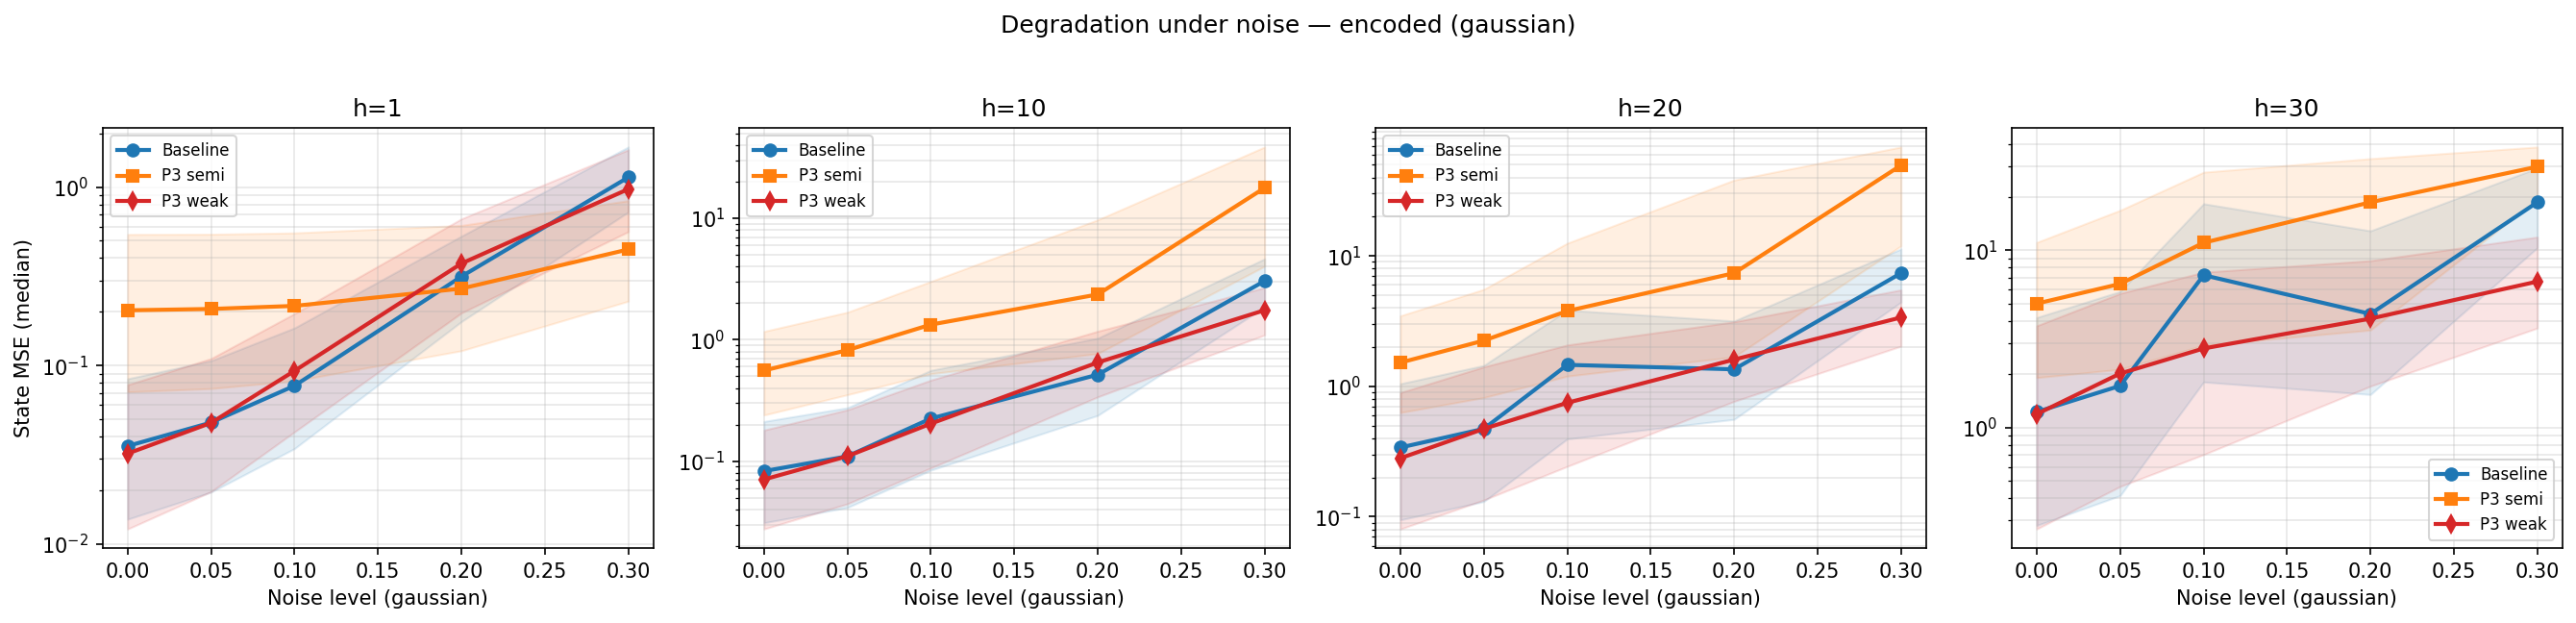
\includegraphics[width=\linewidth]{pics/p3_noise_degradation.png}
    \caption{Αρχή 3 υπό \textlatin{Gaussian noise} (\textlatin{CartPole}). Σε μεγάλους ορίζοντες και υψηλό θόρυβο, η ασθενής επίβλεψη (\textlatin{P3-weak}, κόκκινο) ξεπερνά το πλήρως επιβλεπόμενο \textlatin{Baseline} (μπλε), δρώντας ως έμμεση κανονικοποίηση· η μερική επίβλεψη (\textlatin{P3-semi}) αποτυγχάνει.}
    \label{fig:p3_noise}
\end{figure}

\subsection{\textbf{Αρχή 4: Συμπίεση χωρίς Απώλεια Ποιότητας}}
Η συνθετική αποκωδικοποίηση επιβεβαίωσε τον ισχυρισμό του άρθρου. Στο \textlatin{CartPole}, οι τρεις ανεξάρτητοι αποκωδικοποιητές μείωσαν τις παραμέτρους του \textlatin{decoder} κατά \textbf{75.4\%} (από \textlatin{665k} σε \textlatin{164k}) και τις συνολικές κατά $25.9\%$, διατηρώντας ουσιαστικά ταυτόσημη ποιότητα ανακατασκευής (Πίνακας~\ref{tab:p4}, Σχήμα~\ref{fig:p4}). Η συνιστωσοποιημένη έξοδος προσφέρει επιπλέον δυνατότητα επαλήθευσης ανά αντικείμενο, στοιχείο κρίσιμο για την ασφάλεια.

\begin{table}[h]
\centering
\caption{Αρχή 4: \textlatin{baseline} vs \textlatin{P4} στο \textlatin{CartPole}.}
\label{tab:p4}
\small
\begin{tabular}{l r r}
\toprule
\textlatin{Metric} & \textlatin{Baseline} & \textlatin{P4} \\
\midrule
\textlatin{recon MSE} $\downarrow$ & 0.00315 & 0.00306 \\
\textlatin{SSIM} $\uparrow$ & 0.9581 & 0.9582 \\
\textlatin{decoder params} $\downarrow$ & \textlatin{665k} & \textlatin{164k} ($-75.4\%$) \\
\bottomrule
\end{tabular}
\end{table}

\begin{figure}[h]
    \centering
    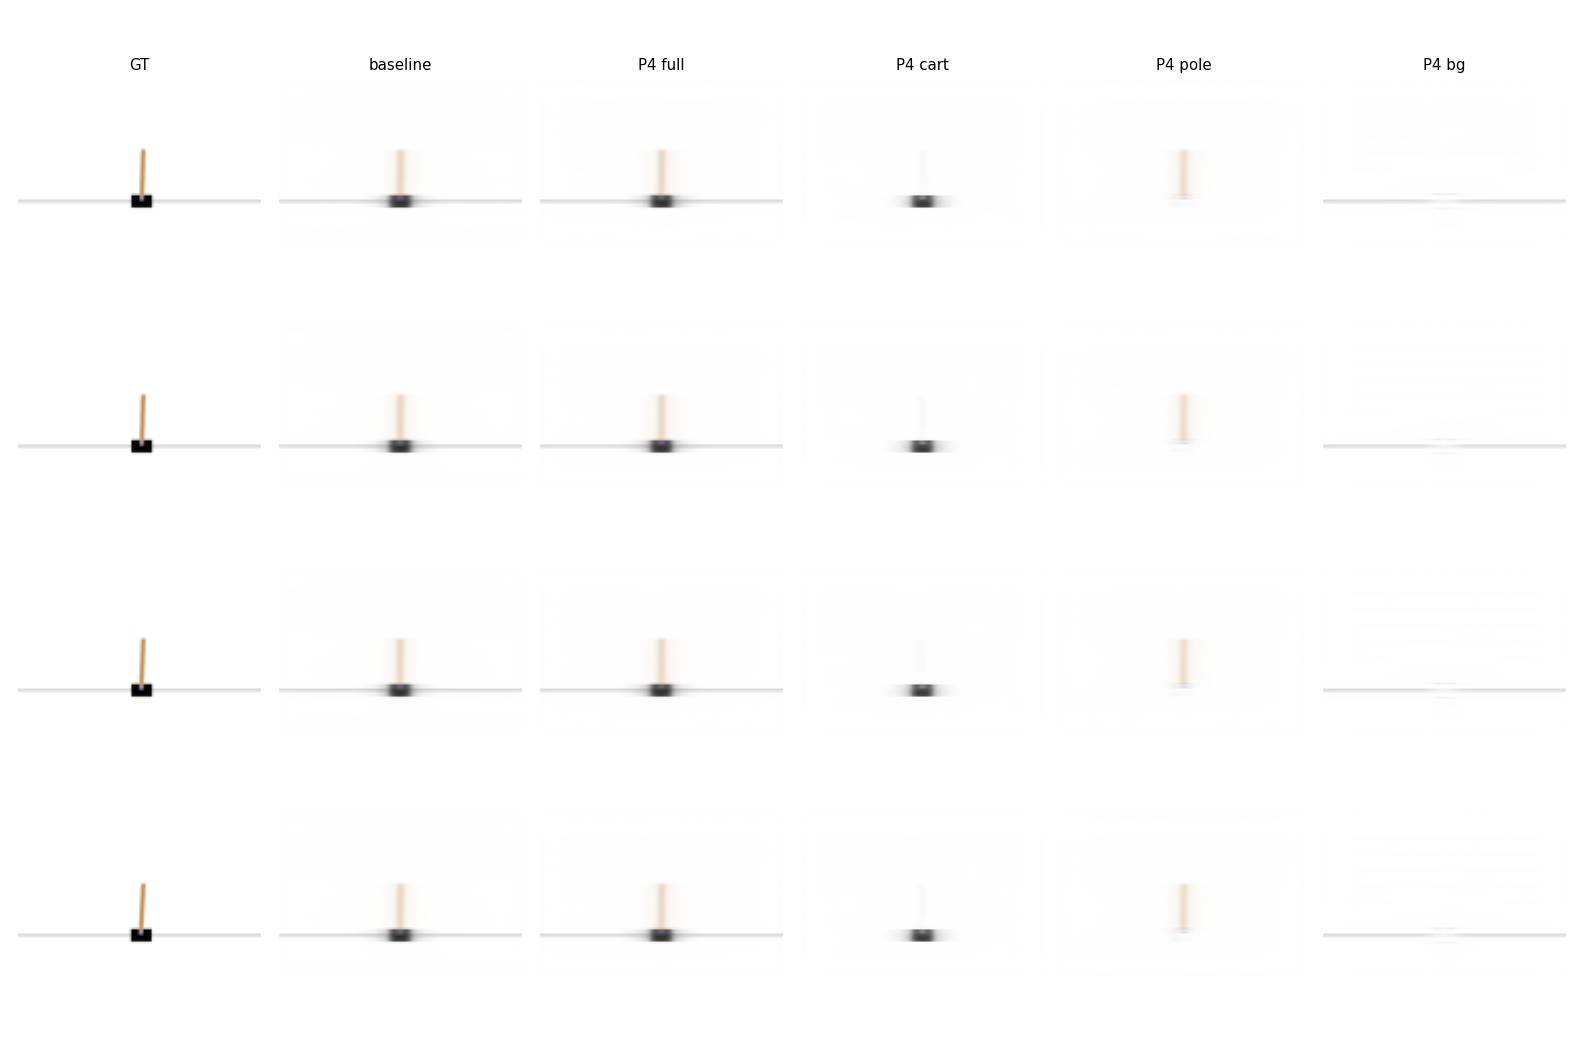
\includegraphics[width=\linewidth]{pics/p4_compare.png}
    \caption{Αρχή 4: \textlatin{GT} vs \textlatin{baseline} vs \textlatin{P4} (σύνθεση και επιμέρους αποκωδικοποιητές \textlatin{cart}/\textlatin{pole}/\textlatin{bg}).}
    \label{fig:p4}
\end{figure}

\subsection{\textbf{Ερμηνεύσιμη Δυναμική: \textlatin{SINDy} vs \textlatin{LSTM}}}
Η αραιή ταυτοποίηση ανέκτησε αυτόματα ερμηνεύσιμες εξισώσεις κίνησης με μόλις 12 μη-μηδενικούς όρους (από 88), συμπεριλαμβανομένων των κινηματικών ολοκληρωμάτων (π.χ. $x_{t+1}=x_t+0.021\,\dot{x}$, $\theta_{t+1}=\theta_t+0.176\,\dot{\theta}$) και του όρου βαρύτητας $\sin\theta$. Στην αξιολόγηση ευρωστίας (Πίνακας~\ref{tab:sindy}), αν και σε καθαρές συνθήκες τα τρία μοντέλα ισοβαθμούν, υπό έντονο θόρυβο ($\sigma=0.30$) το \textlatin{SINDy} υποβαθμίζεται μόλις $\times 3.7$ έναντι $\times 15$ του \textlatin{LSTM}, επιβεβαιώνοντας ότι η ρητή φυσική δομή προσφέρει ευρωστία. Το \textlatin{gray-box hybrid} επιτυγχάνει το χαμηλότερο σφάλμα σε καθαρές συνθήκες, αλλά με μη φραγμένη υπολειμματική διόρθωση κληρονομεί την ευθραυστότητα του \textlatin{LSTM} στον θόρυβο.

\begin{table}[h]
\centering
\caption{Ευρωστία δυναμικής σε \textlatin{Gaussian noise} (\textlatin{mean State MSE}, \textlatin{Baseline} latent).}
\label{tab:sindy}
\small
\begin{tabular}{l r r r}
\toprule
$\sigma$ & \textlatin{LSTM} & \textlatin{SINDy} & \textlatin{Hybrid} \\
\midrule
0.00 & 0.033 & 0.035 & \textbf{0.027} \\
0.10 & 0.085 & \textbf{0.045} & 0.075 \\
0.30 & 0.509 & \textbf{0.130} & 0.441 \\
\bottomrule
\end{tabular}
\end{table}

\section{\textbf{Συζήτηση}}
\label{sec:discussion}
Τα ευρήματά μας υποδεικνύουν ότι ο σχεδιασμός \textlatin{World Models} απαιτεί συμβιβασμούς (\textlatin{trade-offs}). Η σκληρή αρχιτεκτονική δομή (Αρχή 1) είναι η ασφαλέστερη επιλογή απέναντι σε μη δομημένες αλλοιώσεις (π.χ. φθορά αισθητήρων). Η ρητή κανονικοποίηση (Αρχή 2) είναι εξαιρετικά ισχυρή αλλά ταυτόχρονα εύθραυστη αν το περιβάλλον παραβιάσει τις υποθέσεις της. Τέλος, η απαίτηση για τέλεια δεδομένα είναι μύθος: οι προσεγγιστικές μετρήσεις (Αρχή 3) μπορούν πρακτικά να βελτιώσουν την ικανότητα γενίκευσης του μοντέλου εκτός κατανομής.

\section{\textbf{Συμπεράσματα}}
\label{sec:conclusion}
Αναπτυξαμε ένα εύρωστο \textlatin{pipeline} εκπαίδευσης και αξιολόγησης για \textlatin{Physics-Informed World Models}. Μέσω αυστηρών \textlatin{OOD} πειραμάτων, δεν αναπαράγαμε απλώς τη σχετική βιβλιογραφία, αλλά αποκαλύψαμε κρίσιμους, αδημοσίευτους μηχανισμούς σχετικά με το πώς η αποσύνδεση, η ισοδυναμία και η ασθενής επίβλεψη συμπεριφέρονται κάτω από ρεαλιστικό αισθητηριακό θόρυβο. Επιπλέον, δείξαμε ότι η συνθετική αποκωδικοποίηση (Αρχή 4) συμπιέζει τον \textlatin{decoder} κατά $75\%$ χωρίς απώλεια ποιότητας, και ότι η αραιή ταυτοποίηση δυναμικής (\textlatin{SINDy}) εξάγει ερμηνεύσιμες και εύρωστες εξισώσεις κίνησης, ανοίγοντας δρόμο προς δυναμικά μοντέλα που διατηρούν φυσικές εγγυήσεις (π.χ. \textlatin{Hamiltonian NNs}). Τα αποτελέσματα αυτά προσφέρουν πρακτικές οδηγίες για την ανάπτυξη πραγματικών ρομποτικών συστημάτων.

\begin{thebibliography}{00}
\selectlanguage{english}
\bibitem{piwm}
Original PIWM Authors, "World Model Principles", \textit{Conference/Journal Name}, Year.

\bibitem{worldmodels}
D. Ha and J. Schmidhuber, "World Models", \textit{arXiv preprint arXiv:1803.10122}, 2018.

\bibitem{sindy}
S. L. Brunton, J. L. Proctor, and J. N. Kutz, "Discovering governing equations from data by sparse identification of nonlinear dynamical systems", \textit{PNAS}, vol. 113, no. 15, pp. 3932--3937, 2016.
\end{thebibliography}

\end{document}
